\documentclass[runningheads]{llncs}

\usepackage[T1]{fontenc}
\usepackage{graphicx}
\usepackage{svg}
\usepackage[ngerman]{babel}
\usepackage[utf8]{inputenc}
\usepackage[babel, german=guillemets]{csquotes}
\usepackage{mathtools}
\usepackage{xfrac}
\usepackage{multirow}
\usepackage{multicol}
\usepackage[hidelinks]{hyperref}
\usepackage{color}
\usepackage[nolist]{acronym}
\usepackage{listings}
\usepackage{tabularx}
\usepackage{makecell}
\usepackage{pifont}
\renewcommand\UrlFont{\color{blue}\rmfamily}
\newcommand{\cmark}{\ding{51}}

\graphicspath{ {./img/} }

\begin{document}

\title{Apples „Wo ist“ Dienst – Funktionsweise und Missbrauchspotential}


\author{Lukas Panni\inst{1}}

\authorrunning{L. Panni}
\institute{Hochschule Karlsruhe, Karlsruhe}

\maketitle              % typeset the header of the contribution

\begin{abstract}
Apples „Wo ist“ Dienst ermöglicht die Lokalisierung verlorener Geräte.
Dazu senden unterstützte Geräte periodisch Daten über \ac{BLE} an Apple-Geräte in der Nähe.
Diese bestimmen den Standort und senden diesen an Apples Server, von wo der Besitzer des verlorenen Geräts die Daten abrufen kann.
Durch die große Verbreitung von Apple-Geräte ist die Wahrscheinlichkeit hoch, dass \ac{BLE}-Pakete verlorener Geräte ein Apple-Gerät in der Nähe erreichen kann.
Über eine Ende-zu-Ende-Verschlüsselung werden die Standorte zudem vor unberechtigtem Zugriff geschützt.
Die vorliegende Arbeit beschreibt die Funktionsweise des Dienstes und zeigt dabei, welche Schutzmaßnahmen ergriffen werden.
Weiterhin werden konkrete Missbrauchsszenarien aufgezeigt, gegen welche die ergriffenen Maßnahmen nur unzureichend schützen.
Basierend darauf werden notwendige Schutzmaßnahmen vorgeschlagen.
Jedoch kann ohne eine umfassende Anpassung auch mit zusätzlichen Maßnahmen nicht jeder Missbrauch ausgeschlossen werden.
% \keywords{ A \and B \and C }
\end{abstract}

\begin{acronym}[AAAAA]

    \acro{API}[API]{Application Programming Interface}
    \acro{AES}[AES]{Advanced Encryption Standard}
    \acro{BLE}[BLE]{Bluetooth Low Energy}
    \acro{DSGVO}[DSGVO]{Datenschutzgrundverordnung}
    \acro{DOS}[DoS]{Denial of Service}
    \acro{ECC}[ECC]{Elliptic Curve Cryptography}
    \acro{ECDH}[ECDH]{Elliptic Curve Diffie-Hellman}
    \acro{GCM}[GCM]{Galois/Counter Mode}
    \acro{GPS}[GPS]{Global Positioning System}
    \acro{IOT}[IoT]{Internet of Things}
    \acro{KDF}[KDF]{Key Derivation Function}
    \acro{MAC}[MAC]{Media Access Control}
    \acro{MBK}[MBK]{Master Beacon Key}
    \acro{MITM}[MitM]{Man-in-the-Middle}
    \acro{MSB}[MSB]{Most Significant Bit}
    \acro{SHA}[SHA]{Secure Hash Algorithm}
    \acro{TLS}[TLS]{Transport-Layer Security}
    
\end{acronym}


\section{Einleitung}
\subsection{Motivation}
% TODO: Motivation

\cite{Spec_BLE_5.3}
\newpage
\section{Crowdsourced-Tracking: Funktionsweise}
\label{sec:Funktionsweise}

Mit der Einführung ihres ersten \ac{BLE}-Trackers hat die Firma Tile 2013 das Konzept eines \ac{BLE}-basierten Tracking-Systems populär gemacht.
Wie viele konkurrierende Systeme, darunter Apples „Wo ist?“ Dienst, setzt auch Tile auf crowdsourcing zur Bestimmung der Position verlorener Gegenstände \cite{Weller_BLE_Finders}.
Die grundlegende Funktion dieser Systeme ist jeweils identisch und in \autoref{fig:tracker_allgemein} gezeigt: Ein zu findendes Gerät \textit{a)} sendet periodisch \ac{BLE}-Advertisements, die von Smartphones in der Nähe \textit{b)}, welche am entsprechenden System teilnehmen, empfangen werden können \textit{(1)}.
Das zu findende Gerät ist dabei entweder ein Endgerät wie ein Smartphone oder ein Tablet, oder ein spezieller, batteriebetriebener, sogenannter Tracker.
Solche Tracker können an anderen Gegenstände befestigt werden, sodass diese bei Verlust ebenfalls gefunden werden können.
Die Empfänger der \ac{BLE}-Advertisements können ihre Position über das \ac{GPS} bestimmen und diese zusammen mit einer ID, welche das zu findende Gerät identifiziert, an einen Server übermitteln \textit{(2)}.
Der Besitzer des verlorenen Geräts \textit{c)} kann die Position seines Geräts vom Server abrufen \textit{(3)} \cite{Garg_Secure_Tracker}.
Das Funktionsprinzip ist dementsprechend vergleichsweise einfach.
\begin{figure}[ht]
    \centering 
    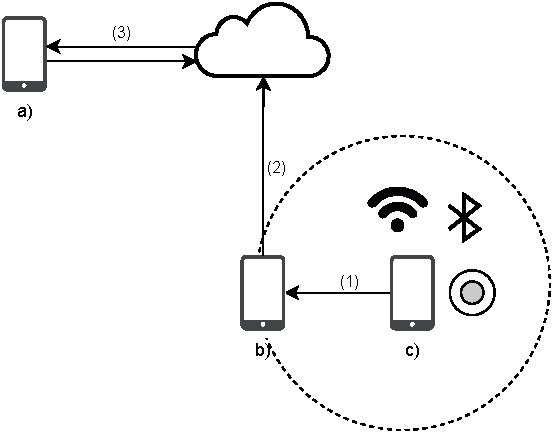
\includegraphics[width=0.9\textwidth]{BLE_Tracker_allgemein.pdf}
    \caption{Allgemeine Funktionsweise des Crowdsourced-Tracking mit \ac{BLE}.}
    \label{fig:tracker_allgemein}
\end{figure}
Qualität und Nützlichkeit für die Nutzer eines solchen Dienstes hängt aber stark von der Anzahl der Nutzer ab.
Die Position eines verlorenen Geräts kann nur vom Tracking-Dienst abgerufen werden, wenn ein Nutzer des gleichen Dienstes ein \ac{BLE}-Advertisement des verlorenen Geräts empfangen und die Position an den Dienst übermittelt hat.
Je mehr Nutzer ein Dienst hat, desto größer die Wahrscheinlichkeit, dass sich ein Nutzer vor kurzem in der Nähe des verlorenen Geräts befand und desto größer die Wahrscheinlichkeit, das verlorene Gerät zu finden.


In allen untersuchten Systemen konnten Weller \textit{et al.} \cite{Weller_BLE_Finders} und Garg \textit{et al.} \cite{Garg_Secure_Tracker} unabhängig voneinander verschiedene Schwachstellen finden, die sowohl Privatsphäre als auch Sicherheit betreffen.
Unter anderem übermittelten einige Dienste die Positionsdaten unverschlüsselt und erlaubten das unberechtigte Abrufen von personenbezogenen Daten über die Backends der Dienste.
Auch zum Veröffentlichungszeitpunkt der Arbeit von Weller \textit{et al.} \cite{Weller_BLE_Finders} waren nicht alle der erkannten Schwachstellen behoben.
Außerdem bot keiner der von Garg \textit{et al.} \cite{Garg_Secure_Tracker} untersuchten Dienste ausreichend Schutz vor dem Melden falscher Positionsdaten.


\subsection{Funktionsweise des „Wo ist?“ Dienstes im Detail}
\label{sec:Funktionsweise_FindMy}
Auf seiner Informationsseite über den „Wo ist?“ Dienst gibt Apple an: „Geräte in der Nähe senden den Standort [...] sicher an iCloud weiter [...]. Zum Schutz der Privatsphäre passiert das alles anonym und verschlüsselt“ \cite{Apple_WoIst}.
Apple erhebt demnach den Anspruch einen Dienst anzubieten, der nicht nur sicherer, sondern auch besser für die Privatsphäre der Nutzer ist als die Dienste der Konkurrenz.
Vergangene Untersuchungen haben allerdings bereits gezeigt, dass auch Apples Dienst einige Schwachstellen aufweist \cite{Heinrich_FindMy,Tonetto_FindMy}.
Diese Schwachstellen werden in \autoref{sec:Missbrauch} wieder aufgegriffen.

Der vermutlich größte Vorteil des Dienstes liegt vermutlich aber in der großen Zahl der Geräte, welche aktiv die Positionsdaten verlorener Geräte sammeln.
Laut Apple nehmen „hunderte[n] Millionen iPhone, iPad und Mac Geräte[n]“ \cite{Apple_WoIst} am „Wo ist?“ Dienst teil.
Der größte Konkurrent Tile hatte im Jahr 2021 laut der bekannten Gadget-Review Webseite \textit{Pocket-Lint} 40 Millionen Nutzer und kann damit für die Lokalisierung auf ein deutlich kleineres Netzwerk zurückgreifen als Apple \cite{Tile_Network}.


Auf Basis des Reverse-Engineering des „Wo ist?“ Dienstes von Heinrich \textit{et al.} in \cite{Heinrich_FindMy} und der Spezifikation für Drittanbieter \cite{Apple_FindMySpec} wird im Folgenden die grundlegende Funktionsweise des Dienstes erläutert.
Dabei wird insbesondere darauf eingegangen, welche Maßnahmen Apple ergreift um Sicherheit und Privatsphäre der Nutzer besser zu schützen als die konkurrierenden Dienste. 

In der Spezifikation werden folgende vier Rollen definiert \cite{Apple_FindMySpec}:
\begin{itemize}
    \item \textbf{Owner Device}: Alle Geräte, in denen die Apple-ID des Besitzers hinterlegt ist.
    \item \textbf{Accessory}: Das zu findende Gerät.
    \item \textbf{Find My network}: Die Menge aller Apple-Geräte, mit aktivierter „Wo ist?“ Funktion. Einzelne Geräte werden jeweils als \textbf{Finder Device} bezeichnet.
    \item \textbf{Apple Server}: Server der die Standortinformationen speichert.
\end{itemize}
\autoref{fig:findMy_roles} zeigt die Rollen, deren Beziehungen und die jeweiligen Aufgaben wie in der Spezifikation angegeben.
\begin{figure}
    \centering
    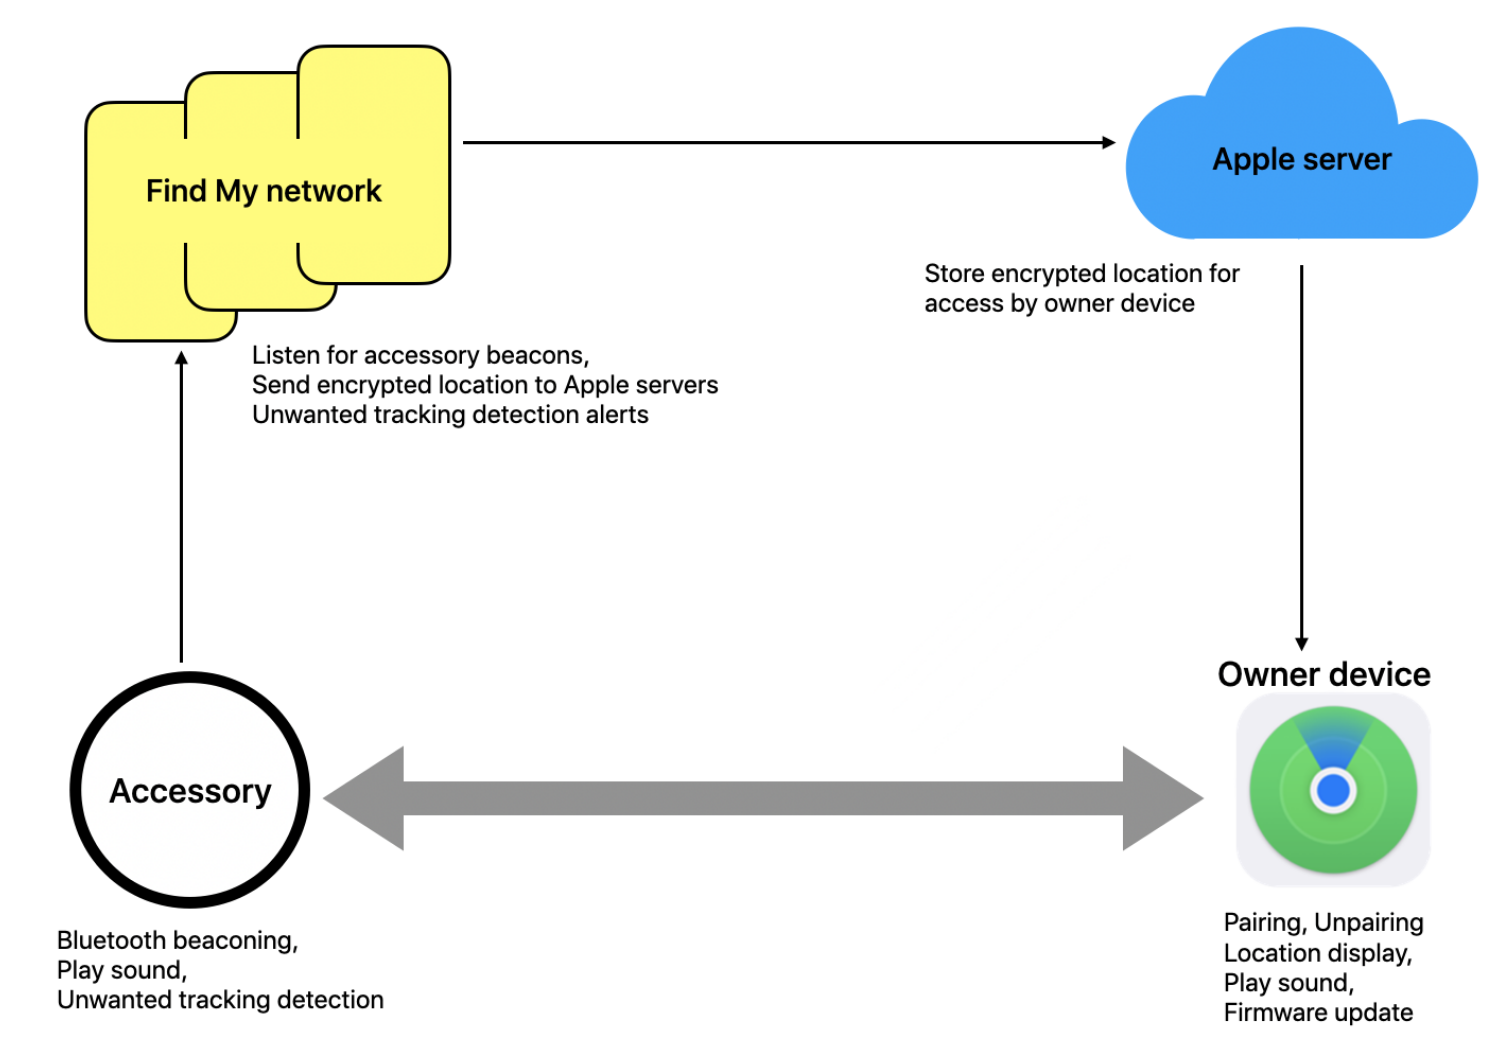
\includegraphics[width=0.9\textwidth]{findMy_roles}
    \caption{Rollen im „Wo ist?“ Dienst \cite{Apple_FindMySpec}.}
    \label{fig:findMy_roles}
\end{figure}
Apple erlaubt seit April 2021 auch Drittanbietern die Nutzung des „Wo ist?“ Netzwerks um die eigenen Produkte zu finden \cite{Apple_FindMy3rdParty}.
Da die Spezifikation speziell für Drittanbieter erstellt wurde, wird das zu findende Gerät als \textit{Accessory} bezeichnet.
In der folgenden Beschreibung wird jedoch der Begriff \textit{Lost Device} verwendet, der auch von Heinrich \textit{et al.} \cite{Heinrich_FindMy} verwendet wird und sowohl Produkte von Drittanbietern als auch von Apple abdeckt.
Das zu findende Gerät muss mit der Apple-ID des Besitzers verbunden sein, um gefunden werden zu können.
Drittanbieter Geräte und AirTags müssen dazu vor der ersten Verwendung über einen Pairing-Prozess mit einem Apple-Gerät verbunden werden \cite{Apple_FindMySpec}.

\subsubsection{Kryptografie}
\label{sec:Kryptografie}

Um bessere Sicherheit und Privatsphäre als die Konkurrenz zu bieten, setzt Apple auf asymmetrische \ac{ECC} Verschlüsselung.
Standortdaten werden immer Ende-zu-Ende verschlüsselt, sodass potenzielle Angreifer die Positionen der Nutzer nicht verfolgen können, sollten sie an Standortdaten gelangen.
Durch den verwendeten Prozess zur Verschlüsselung kann auch Apple selbst nicht auf die Standortdaten zugreifen.
Nur der Besitzer des Geräts kann die Standortdaten zur Lokalisierung des Geräts entschlüsseln \cite{Greenberg_FindMyCrypto}.


Jedes Owner Device erstellt zunächst den sogenannten \textit{Master Beacon Key}, bestehend aus einem \ac{ECC} Schlüsselpaar und einem symmetrischen Schlüssel.
Diese Schlüssel werden über den iCloud Dienst zwischen allen Geräten mit der gleichen Apple-ID synchronisiert.
Um die Schlüssel bei der Synchronisierung zu schützen, werden sie mit einem symmetrischen Schlüssel, aus der als sicher geltenden iCloud Keychain, verschlüsselt \cite{Heinrich_FindMy,Afonin_iCloudKeychain}.
Der private Schlüssel des \ac{ECC}-Schlüssels sowie der symmetrische Schlüssel des Master Beacon Keys müssen geheim bleiben.
Auch der öffentliche Teil des \ac{ECC}-Schlüssels im Master Beacon Key, wird nie über \ac{BLE} übertragen.
Stattdessen wird der Master Beacon Key verwendet, um temporär gültige Schlüssel abzuleiten, die im \ac{BLE}-Advertising übertragen werden können.
Für die Ableitung dieser sogenannten \textit{Advertising Keys} wird die ANSI X9.63-\ac{KDF} verwendet \cite{Apple_FindMySpec}.
Aus einem im \ac{BLE}-Advertising übertragenen öffentlichen Schlüssel kann somit, ohne Kenntnis des Master Beacon Keys, der nächste öffentliche Schlüssel nicht abgeleitet werden.
Durch regelmäßiges Wechseln des verwendeten Avertising Keys wird es einem Angreifer erschwert, ein Lost Device anhand der im Advertising übertragenen Daten zu verfolgen.
Da für die Verschlüsselung der Standortdaten nur die X-Koordinate des öffentlichen Schlüssels benötigt wird, kann auf die Übertragung der Y-Koordinate verzichtet werden \cite{Heinrich_FindMy}.

Die Verschlüsselung der Standortdaten erfolgt auf dem Finder Device mit dem \ac{AES}-Algorithmus im \ac{GCM}-Modus.
Aus dem, vom Finder Device empfangenen, Advertising Key wird ein temporäres \ac{ECC}-Schlüsselpaar generiert, aus welchem über einen \ac{ECDH} Schlüsselaustauch ein geteiltes Geheimnis generiert und durch die Anwendung der ANSI X9.63-\ac{KDF} ein symmetrischer Schlüssel abgeleitet wird.
Der Schlüsselaustausch verwendet den privaten Teil des temporären \ac{ECC}-Schlüssels und den öffentlichen Teil des empfangenen Advertising Keys.
Von diesem werden die ersten 16 Byte als Schlüssel für den \ac{AES}-Algorithmus und die folgenden 16 Byte als Initialisierungsvektor verwendet \cite{Heinrich_FindMy}.
Durch die Ausführung der Verschlüsselung auf dem Finder Device, kann die Batterie des Lost Devices geschont werden und die Lokalisierung verlorener Geräte bleibt länger möglich.
Insbesondere bei AirTags oder Produkten von Drittanbietern kann das hilfreich sein, da diese Geräte, eine im Vergleich zu einem iPhone oder iPad, sehr geringe Batteriekapazität haben.
Die kryptografischen Funktionen könnten den Stromverbrauch der Geräte deutlich erhöhen, wenn bei jedem Kontakt mit einem Finder-Device dieser komplexe Verschlüsselungsprozess ablaufen muss.
Durch die Verschlüsselung auf den Finder Devices müssen die Lost Devices nur alle 15 Minuten einen neuen Schlüssel ableiten, was durch die geringere Zahl der Operationen eine deutlich geringere Belastung für die Batterie darstellt.


Für die Entschlüsselung kann das geteilte Geheimnis über den \ac{ECDH} Schlüsselaustausch mit dem öffentlichen Teil des temporären Schlüssels und dem privaten Teil des Advertising Keys berechnet werden.
Der symmetrische Schlüssel entsteht wieder durch die Anwendung der ANSI X9.63-\ac{KDF} auf das geteilte Geheimnis.
Damit ist sichergestellt, dass die verschlüsselten Daten nur vom Besitzer entschlüsselt werden können.
Dieser kann die für das Advertisement verwendeten Schlüsselpaare unabhängig vom verlorenen Gerät aus dem Master Beacon Key ableiten und hat somit Zugriff auf die privaten Schlüssel.
Der öffentliche Teil des temporären Schlüssels und ein \ac{SHA}-256 Hash des verwendeten Advertisement Keys wird mit den verschlüsselten Daten auf Apples Server hochgeladen.
Der Besitzer kann diese Daten abrufen und aus der Kombination des öffentlichen temporären Schlüssels und dem privaten Advertisement Keys das geteilte Geheimnis und somit den symmetrischen Schlüssel berechnen \cite{Heinrich_FindMy}.

Da Geräte ohne Internetverbindung, wie zum Beispiel AirTags oder andere Geräte von Drittanbietern, die Master Beacon Keys nicht über die iCloud Synchronisation erhalten können, müssen diese Geräte auf andere Weise an einen initialen Schlüssel kommen.
% TODO: Schlüsselaushandlung, Infos aus Spec

\subsubsection{Ablauf beim Verlust eines Geräts}
\label{sec:Verlust}

Alle Apple Geräte mit aktivierter Bluetooth-Funktion, die für das Finden durch den „Wo ist?“ Dienst angemeldet sind, senden periodisch, in der Regel im Advertising Intervall von 2 s \ac{BLE}-Advertisements.
Die im Advertisement enthaltenen Daten unterscheiden sich jedoch abhängig vom Zustand des Geräts.
iPhones, iPads und MacBooks mit Internetverbindung und alle unterstützen Geräte mit einer aktiven \ac{BLE}-Verbindung mit einem Owner Device, gelten nicht als Lost Device und senden deshalb nur die ersten fünf Bytes des öffentlichen Advertisement Keys.
Das Advertisement erfolgt vermutlich um erkennen zu können, wenn ein Gerät in der Nähe die Verbindung verliert.
Die ersten fünf Byte des öffentlichen Schlüssels sollten in der Regel ausreichen um verschiedene Geräte voneinander unterscheiden zu können.
Vermutlich werden Funktionen, wie die Warnung beim Zurücklassen eines Geräts \cite{Apple_FindMyWarning}, über diese Advertisement Daten umgesetzt.

Sobald ein Gerät die Internetverbindung oder die \ac{BLE}-Verbindung zum Owner Device verliert, wird es als Lost Device angesehen.
Um in diesem Zustand von anderen Finder Devices gefunden zu werden, beginnt das Lost Device \ac{BLE}-Advertisements mit dem kompletten öffentlichen Advertisement Key zu senden \cite{Apple_FindMySpec}.
Die Advertisement Pakete werden immer mit dem Typ \textit{manufacturer-specific data} gesendet, sodass neben angebotenen \ac{BLE}-Services auch eigene Daten übertragen werden können.
Das Format erlaubt nach einer Firmen-ID von zwei Byte, maximal 27 weitere Byte zu übertragen.
Da Apple, die manufacturer-specific data auch für andere Zwecke, wie zum Beispiel AirDrop nutzt, wird jeweils ein weiteres Byte für den Typ ($0x12$) des Pakets und dessen Länge verwendet.
Zur Identifikation des Lost Device und zur Verschlüsselung der Standortdaten müssen die 28 Byte der X-Koordinate des aktuellen öffentlichen Schlüssels im Advertisement übertragen werden \cite{Heinrich_FindMy}.
Jeder Schlüssel wird für 15 Minuten verwendet, um die Verfolgung des Geräts anhand der Advertising-Daten für Dritte zu erschweren.
Nach Ablauf der 15 Minuten wird ein neuer Schlüssel abgeleitet und für die nächste Periode im Advertisement versendet.
Da der Schlüssel aus dem Advertising alleine nicht reicht, um den nächsten Schlüssel abzuleiten, kann so die Privatsphäre im Vergleich zu Konkurrenzprodukten verbessert werden.
Die 25 Byte Payload reichen nicht aus, um die X-Koordinate des öffentlichen Schlüssels zu übertragen.
Deshalb  wird zusätzlich die Advertising Address des Advertisement Pakets ausgenutzt.
Die Advertising Address kann zum Schutz der Privatsphäre laut \ac{BLE}-Spezifikation \cite{Spec_BLE_5.3} von der tatsächlichen \ac{MAC}-Adresse des Geräts abweichen.
Üblicherweise wird diese Funktion verwendet um über zufällige \ac{MAC}-Adressen die Nachverfolgbarkeit von Geräten und Rückschlüsse auf den Gerätehersteller zu erschweren.
Durch Codierung von Daten in der zufälligen Adresse, kann das Feld jedoch für den Transfer beliebiger Daten ausgenutzt werden.
Apple speichert die ersten 46 Bit des öffentlichen Schlüssels in der Advertising Address, wobei die beiden \acp{MSB} des ersten Bytes jeweils auf 1 gesetzt werden müssen, um der \ac{BLE}-Spezifikation zu genügen \cite{Heinrich_FindMy}.
Die restlichen 170 Bit bestehend aus den Bytes 6 bis 27 und den fehlenden zwei Bits des Byte 0 werden im Advertising Payload übertragen \cite{Apple_FindMySpec}.
\autoref{fig:apple_advertising} zeigt den resultierenden Aufbau eines Advertisement Pakets des „Wo ist?“ Dienstes.
Die Teile, in welchen der öffentliche Schlüssel übertragen wird, sind gelb hinterlegt.
Das als "Hint" bezeichnete Feld codiert laut Spezifikation \cite{Apple_FindMySpec} Byte 5 des öffentlichen Schlüssels, laut Heinrich \textit{et al.} \cite{Heinrich_FindMy} ist dieses Feld bei iOS immer 0.
Mit einem eigenen \ac{BLE}-Scan konnte beobachtet werden, dass das Feld bei einem iOS-Gerät auf 0 gesetzt war, obwohl Byte 5 des öffentlichen Schlüssels ungleich 0 war.
Dementsprechend wird dieses Byte vermutlich nur bei Drittanbieter-Produkten und eventuell bei AirTags verwendet.
% TODO: test mit Airtag?
\begin{figure}
    \centering
    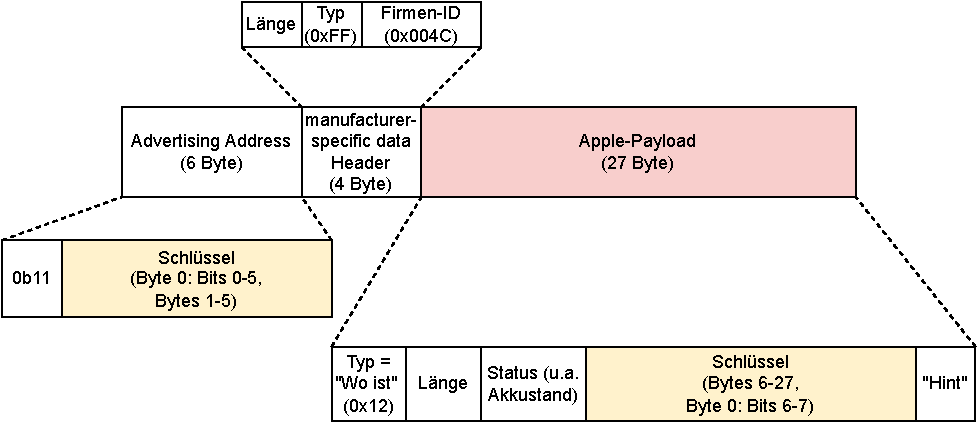
\includegraphics[width=0.9\textwidth]{apple_advertising.pdf}
    \caption{Aufbau der Advertisement Pakete des „Wo ist?“ Dienstes.}
    \label{fig:apple_advertising}
\end{figure}

Standardmäßig scannen alle Apple-Geräte (Finder-Devices) im Hintergrund nach Advertisements, die die Firmen-ID von Apple enthalten.
Wird ein Paket durch den Apple Payload Typ $0x12$ als Advertisement für den „Wo ist?“ Dienst identifiziert, wird vom Finder Device zunächst die aktuelle Position bestimmt und ein sogenannter \textit{Location Report} erstellt.
Das Format dieses Reports ist in \autoref{fig:location_report} gezeigt.
\begin{figure}
    \centering
    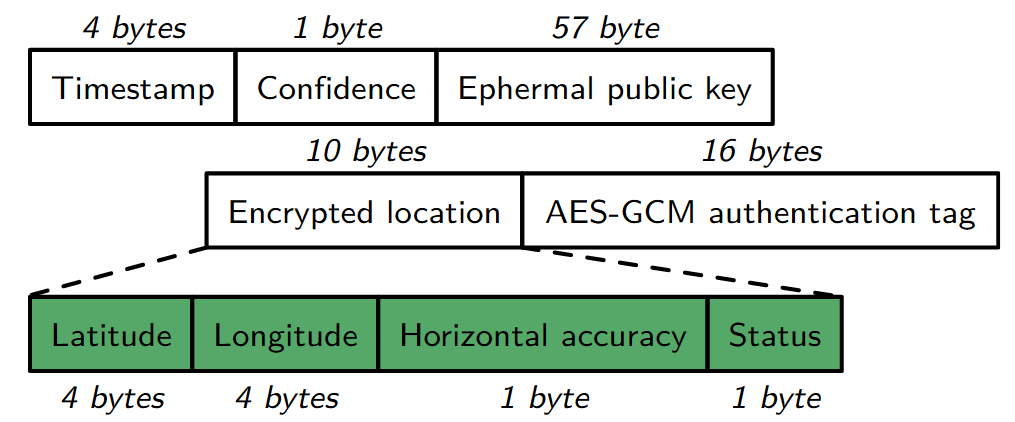
\includegraphics[width=0.85\textwidth]{location_report}
    \caption{Format des Location Reports \cite{Heinrich_FindMy}}
    \label{fig:location_report}
\end{figure}
Der Hauptbestandteil des Reports sind die wie oben beschrieben verschlüsselten Standortinformationen, bestehend aus Koordinaten, Genauigkeit und Status.
Außerdem sind sowohl der temporäre Schlüssel, welcher vom Finder-Device aus dem Advertisement Key abgeleitet und für den \ac{ECDH}-Schlüsselaustausch genutzt wurde, und der \ac{AES}-\ac{GCM} Authentication Tag teil des Reports.
Daneben findet sich unter anderem der Zeitstempel zum Zeitpunkt der Erstellung des Reports.
Beim Upload wird der Report mit einem \ac{SHA}-256 Hash des verwendeten Advertisement Keys verknüpft, um die Identifizierung zu ermöglichen \cite{Heinrich_FindMy}.
Im Vergleich zu konkurrierenden Diensten ist die Verschlüsselung ein wichtiger Schritt, um die Sicherheit und Privatsphäre des Dienstes zu verbessern.
Meist werden Reports nicht unmittelbar nach der Erstellung hochgeladen.
Stattdessen sammelt das Gerät mehrere Reports und lädt diese gebündelt hoch.
Der empfangende Server ordnet den Reports zusätzlich den Zeitstempel zum Zeitpunkt des Datenempfangs zu.
Tonetto \textit{et al.} \cite{Tonetto_FindMy} haben gezeigt, dass die Art der Internetverbindung beeinflusst, wann die Reports hochgeladen werden.
So liegt der Median für den Upload eines Reports bei aktiver WLAN-Verbindung bei 15 Minuten während bei aktiver Mobilfunkverbindung der Median bei 3 Stunden liegt.
Der Upload erfolgt über einen HTTPS-Request, der zusätzlich über den Header authentifiziert wird.
Dieser Header enthält unter anderem ein Identitäts-Zertifikat des Geräts und eine Signatur des Requests.
Diese Signatur wird mit dem privaten Schlüssel erstellt, welcher in einem speziellen Sicherheitsbereich, dem \textit{Secure Enclave Processor} des Geräts gespeichert ist, welcher das unberechtigte Auslesen verhindert.
Somit kann vermutlich sichergestellt werden, dass nur Apple Geräte in der Lage sind Reports hochzuladen, was das Erstellen gefälschter Reports erschwert \cite{Heinrich_FindMy}.


Um die Standortdaten vom Server abzurufen, wird ein über Basic Authentication mit der Apple-ID des Nutzers und einem Token authentifizierter, HTTPS-Request verwendet.
Die Anfrage enthält zusätzlich eine Liste der letzten Advertisement Keys des verlorenen Geräts.
So können die verschlüsselten Location Reports heruntergeladen und anschließend auf dem Gerät entschlüsselt werden, um das verlorene Gerät zu lokalisieren \cite{Heinrich_FindMy}.
\autoref{lst:findmy_result} zeigt die Struktur der Antwort auf einen solchen Request in gekürzter Form.
Die Antwort besteht aus einem Array von Objekten, die jeweils den Hash des Advertisement Keys, einen verschlüsselten Location Report und Metadaten, darunter den Zeitstempel des Datenempfangs, enthalten.
Anhand des Hashes kann der für die Entschlüsselung zu verwendende Advertising Key bestimmt werden.
Entschlüsselte Standortdaten aus mehreren Reports können kombiniert werden, um Genauigkeit bei der Positionsermittlung zu erhöhen.
Gleichzeitig können die Daten mehrerer Reports auch dazu verwendet werden, den Pfad des verlorenen Geräts zu rekonstruieren.
Dafür können bis zu sieben Tage alte Positionen vom Server abgerufen werden \cite{Heinrich_FindMy}.

\begin{lstlisting}[label=lst:findmy_result,caption={Beispielhafte Antwort beim herunterladen von Location Reports\cite{Heinrich_FindMy}.}]
{
    "results": 
    [
        {
            "datePublished": 1586804587284,
            "payload": "JETtmwIEzRBG ....",
            "description": "found",
            "id": "B6E5tpUPbuudAc ...",
            "statusCode": 0
        },
        ...
    ] ,
    "statusCode": "200"
}
\end{lstlisting}
\section{Missbrauch des „Wo ist?“ Dienstes}
\label{sec:Missbrauch}

Das Hauptangriffsziel für Angreifer des „Wo ist?“ Dienstes sind die Standortdaten der Nutzer.
Apple ergreift verschiedene Maßnahmen, um die Sicherheit der Standortdaten sicherzustellen, wie bei der Erläuterung der Funktionsweise in \autoref{sec:Funktionsweise_FindMy} bereits gezeigt wurde.
Untersuchungen, wie durch Tonetto \textit{et al.} \cite{Tonetto_FindMy} haben jedoch geyeigt, dass dennoch Missbrauchspotenzial besteh, gegen welches der Dienst nicht oder nicht ausreichend geschützt ist.
Zunächst werden in \autoref{tab:cia_findmy} die allgemeinen Sicherheitsziele Vertraulichkeit (\textit{Confidentiality}), Integrität (\textit{Integrity}) und Verfügbarkeit (\textit{Availability}) sowie mögliche Angriffsziele im Kontext des „Wo ist?“ Dienstes erklärt.
Darauf aufbauend wird gezeigt, wie die von Apple implementierten Sicherheitsmaßnahmen, viele Angriffsszenarien erfolgreich unterbinden können.
Im Anschluss werden in \autoref{sec:szenarien} konkrete Missbrauchsszenarien aufgezeigt werden, gegen welche Apple nur unzureichende Maßnahmen ergreift und welche somit die Sicherheit und Privatsphäre der Nutzer und sogar Dritter gefährden können.
Diese Szenarien werden in \autoref{sec:Gegenmassnahmen} wieder aufgegriffen und mögliche Gegenmaßnahmen durch Apple respektive die Nutzer vorgestellt.

\begin{table}[h]
  \caption{Sicherheitsziele des „Wo ist?“ Dienstes und mögliche Angriffsziele.}
  \label{tab:cia_findmy}
  \begin{tabularx}{\textwidth}{ |l|X|X| }
    \hline
    \textbf{Sicherheitsziel}  & \textbf{Beschreibung}                                               & \textbf{Angriffsziel}                                           \\
    \Xhline{0.5mm}
    \hline
    Vertraulichkeit           & Standortdaten sind nur befugten Personen zugänglich.                & Standort eines Nutzers oder eines Geräts erhalten.              \\
    \hline
    Integrität                & Standortdaten sind vor Manipulation geschützt.                      & Standortdaten eines Nutzers oder eines Geräts manipulieren.     \\
    \hline
    Verfügbarkeit             & Standortdaten können abgerufen werden.                              & Verhindern, dass Standortdaten abgerufen werden können.         \\
    \hline
  \end{tabularx}
\end{table}

Die von Heinrich \textit{et al.} \cite{Heinrich_FindMy} identifizierten Angreifermodelle in \autoref{fig:adversary_models} zeigen verschiedene Möglichkeiten, wie ein Angreifer versuchen kann, den Dienst anzugreifen.
Sie gehen von vier verschiedenen Angreifermodellen aus, die sich im Angriffsvektor unterscheiden.
Potenzielle Angriffe können demnach von lokal installierten Anwendungen, Geräten in \ac{BLE}-Reichweite, einem klassischen Netzwerkangreifer und dem Dienstanbieter, also von Apple ausgehen.
Für jeden Angriffsvektor werden verschiedene mögliche Ziele definiert.
\begin{figure}[ht]
  \centering
  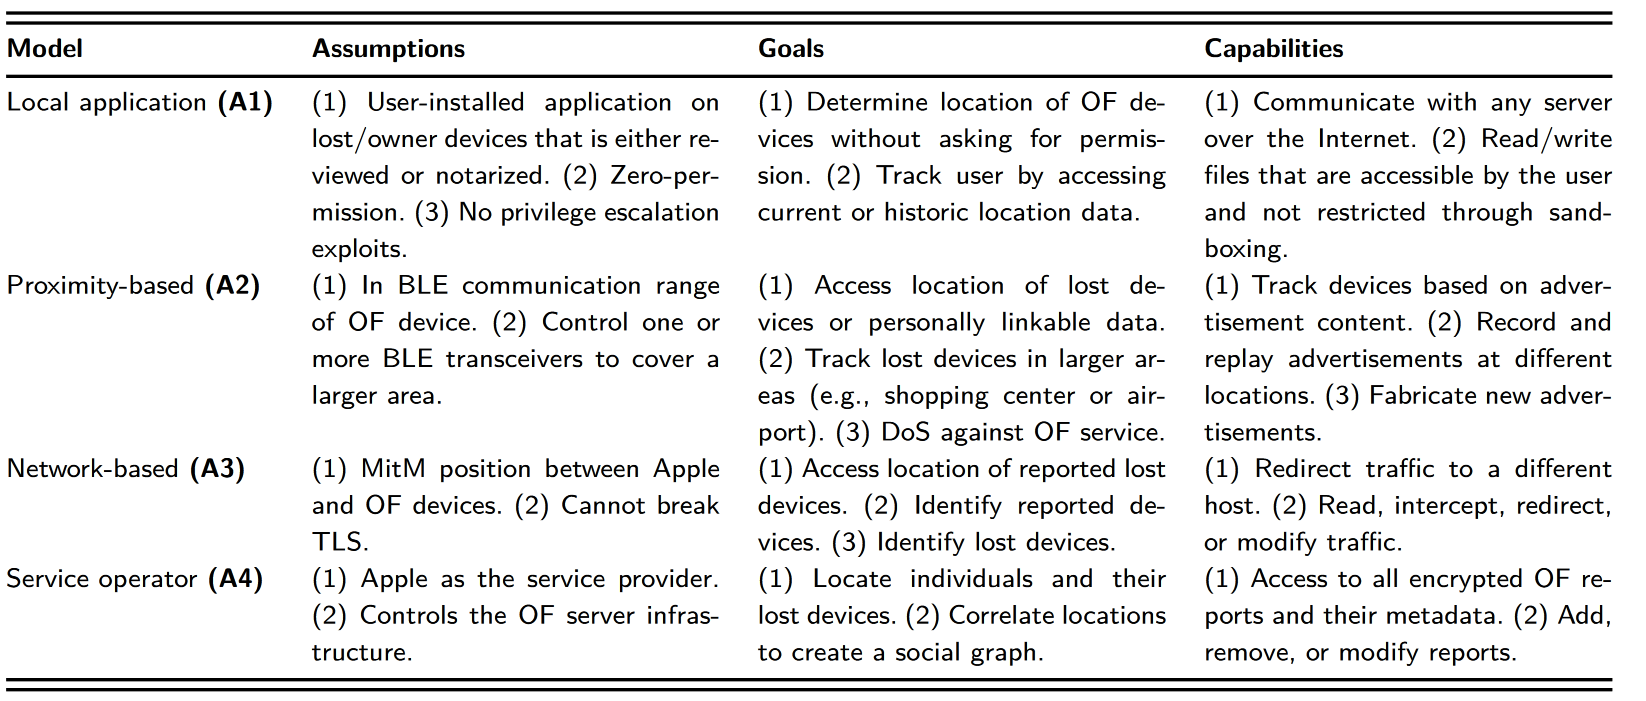
\includegraphics[width=\textwidth]{img/adversary_models}
  \caption{Angreifermodelle für den „Wo ist?“ Dienst \cite{Heinrich_FindMy}.}
  \label{fig:adversary_models}
\end{figure}

\autoref{tab:cia_adversary_models} ordnet den Zielen der einzelnen Angreifermodelle die betroffenen Sicherheitsziele zu.
\begin{table}[h]
  \caption{Zuordnung der Ziele der Angreifermodelle zu den allgemeinen Sicherheitszielen.}
  \label{tab:cia_adversary_models}
  \centering

  \begin{tabularx}{\textwidth}{ |l|X|X|l|X| }
    \hline
    \textbf{Angreifermodell}  & \textbf{Ziel} & \textbf{Vertraulichkeit} & \textbf{Integrität} & \textbf{Verfügbarkeit} \\
    \Xhline{0.5mm}
    \hline
    \multirow{2}{*}{A1} & (1) & \cmark & & \\
    \cline{2-5}
    & (2) & \cmark & & \\
    \hline
    \multirow{3}{*}{A2} & (1) & \cmark & & \\
    \cline{2-5}
    & (2) & \cmark & & \\
    \cline{2-5}
    & (3) & & & \cmark  \\
    \hline
    \multirow{3}{*}{A3} & (1) & \cmark & & \\
    \cline{2-5}
    & (2) & \cmark & & \\
    \cline{2-5}
    & (3) & \cmark & & \\
    \hline
    \multirow{2}{*}{A1} & (1) & \cmark & & \\
    \cline{2-5}
    & (2) & \cmark & & \\
    \hline
  \end{tabularx}
\end{table}
Dabei fällt auf, dass der Fokus auf der Vertraulichkeit der Daten liegt.
Sollten Angreifer Zugriff auf die Standortdaten erhalten, könnten sie diese für viele verschiedene Zwecke missbrauchen.
Zum Beispiel können diese Daten für gezielte Diskriminierung, Verfolgung und Überwachung durch Dritte oder auch durch staatliche Akteure verwendet werden.
Als personenbezogene Daten unterliegen die Standortdaten zusätzlich der \ac{DSGVO}.
Durch mögliche Rückschlüsse auf beispielsweise religiöse oder politische Überzeugungen sind Standortdaten nach Artikel 9 \ac{DSGVO} häufig auch als sensible personenbezogene Daten zu betrachten.
Deshalb ist Apple zumindest innerhalb der Europäischen Union auch verpflichtet, die Vertraulichkeit der Daten durch geeignete Maßnahmen zu schützen.
Wie bereits in \autoref{sec:Funktionsweise_FindMy} gezeigt, trifft Apple verschiedene Maßnahmen, die darauf abzielen die Vertraulichkeit zu wahren.
Die Auswirkungen dieser Maßnahmen werden in \autoref{sec:auswirkungen_sicherheitsmassnahmen} näher betrachtet.
Darüber hinaus werden in \autoref{sec:szenarien} mögliche Angriffe auf die Vertraulichkeit beschrieben, gegen welche die Sicherheitsmaßnahmen von Apple nicht ausreichend schützen.

Angriffe auf die Integrität und die Verfügbarkeit der Daten werden \cite{Heinrich_FindMy} nicht detailliert untersucht.
Nur das \textit{Proximity-based} Modell (A2 in \autoref{tab:cia_adversary_models}) zielt auch auf die Verfügbarkeit der Daten ab.
Wird die Verfügbarkeit beeinträchtigt, ist es für den Besitzer eines Geräts nicht mehr möglich, die aktuellen Standortdaten abzurufen.
Die Beeinträchtigung der Integrität der Daten wird nicht untersucht.
Jedoch ist ein gewisser Zusammenhang mit der Verfügbarkeit gegeben.
Durch gezielte Manipulation der Daten kann der Besitzer beispielsweise nicht mehr unterscheiden welche Daten korrekt sind, was die Verfügbarkeit stark beeinträchtigen kann.
Inwieweit Apples Sicherheitsmaßnahmen auch Integrität und Verfügbarkeit schützen, und welche Angriffe dennoch möglich sind, wird in \autoref{sec:auswirkungen_sicherheitsmassnahmen} und \autoref{sec:szenarien} näher betrachtet.


\subsection{Auswirkungen der Sicherheitsmaßnahmen}
\label{sec:auswirkungen_sicherheitsmassnahmen}

\subsubsection{Ende-zu-Ende Verschlüsselung}
Die Betrachtung der Funktionsweise in \autoref{sec:Funktionsweise_FindMy} zeigt, wie die Ende-zu-Ende-Verschlüsselung des Dienstes technisch umgesetzt wird.
Durch die Verwendung dieses Verschlüsselungsmechanismus kann unter der Annahme, dass der Angreifer die Verschlüsselung nicht brechen kann, gewährleistet werden, dass nur der Besitzer eines verlorenen Geräts die Standortdaten entschlüsseln kann.
Sollte einem Angreifer gelingen die Daten direkt von Apples Server abzurufen, oder über einen \ac{MITM} Angriff die verschlüsselten Daten zu erhalten, können diese ohne die nur auf den Owner Devices verfügbaren Schlüssel nicht entschlüsselt werden.
Dabei werden ein \ac{MITM}-Angriffe durch die Verwendung von \ac{TLS} mit Certificate Pinning bei der Kommunikation mit Apples Servern verhindert \cite{Heinrich_FindMy}.
Durch die Ende-zu-Ende Verschlüsselung werden alle vom Netzwerkangreifer (A3 in \autoref{fig:adversary_models}) ausgehenden Bedrohungen adressiert.
Die zur Entschlüsselung benötigten Schlüssel werden auf den Geräten des Besitzers in der als sicher geltenden iCloud Keychain gespeichert.
So werden auch die von lokalen Angreifern (A1 in \autoref{fig:adversary_models}) ausgehenden Bedrohungen behandelt.
Eine in \cite{Heinrich_FindMy} aufgedeckte Schwachstelle, die aufgrund von unsicherer Speicherung der Schlüssel unbefugten Zugriff auf die Standortdaten ermöglicht, wurde durch Apple mittlerweile behoben.
Zusätzlich wird es durch die Ende-zu-Ende-Verschlüsselung auch Apple unmöglich gemacht, auf die Standortdaten der Nutzer zuzugreifen, womit das Lokalisieren durch den Dienstanbieter (A4 mit Ziel (1) in \autoref{fig:adversary_models}) verhindert wird.
Außerdem verbessert die Verschlüsselung die Integrität der Daten, da einmal verschlüsselte Daten ohne Entschlüsselung nicht manipuliert werden können, ohne dass diese Manipulation erkannt werden kann.
Jedoch ist es möglich, dass die Standortdaten auf Basis eines Replay-Angriffes generiert wurden.
Auf dieses Szenario wird in \autoref{sec:szenarien} näher eingegangen.


\subsubsection{Schlüsselrotation}
Die Schlüsselrotation der Advertising Keys im Intervall von 15 Minuten bei Endgeräten und bis zu 24 Stunden bei Accesories, wie in \autoref{sec:Funktionsweise_FindMy} beschrieben, trägt ebenfalls zur Vertraulichkeit der Standortdaten bei.
Durch die regelmäßige Rotation der Schlüssel wird das Tracking von Geräten anhand der im Advertising gesendeten Daten erschwert.
Damit richtet sich diese Maßnahme gezielt gegen das Tracking durch einen Angreifer in der Nähe (A2 mit Ziel (2) in \autoref{fig:adversary_models}).
Außerdem müssten für einen solchen Angriff viele scannende Geräte so positioniert werden, dass auch bei Bewegung die Advertisement Pakete des zu verfolgenden Geräts von einem der Scanner erfasst wird.
Um größere Bereiche abzudecken, wären jedoch sehr viele scannende Geräte notwendig, was den Angriff bereits deutlich erschwert.
In Verbindung mit der Schlüsselrotation ist die Verfolgung, auch mit hohem Aufwand, nur für das Intervall der Schlüsselrotation möglich.
Allerdings können AirTags und Drittanbieterprodukte durch das längere Intervall für bis zu 24 Stunden über einen solchen Angriff verfolgt werden.
Für Angreifer ist der Angriff jedoch insgesamt so komplex, dass eine direkte Verfolgung des Opfers in den meisten Fällen praktikabler wäre.
Heinrich \textit{et al.} \cite{Heinrich_FindMy} betrachten die Schlüsselrotation als ausreichend, um die Verfolgung von Geräten nach diesem Muster zu verhindern.
Jedoch waren zum Zeitpunkt ihrer Analyse keine Geräte mit einem Intervall der Schlüsselrotation von mehr als 15 Minuten auf dem Markt.


\subsection{Missbrauchsszenarien ohne ausreichende Gegenmaßnahmen}
\label{sec:szenarien}

Im Folgenden sind sieben Missbrauchsszenarien aufgeführt, welche nicht ausreichend durch Gegenmaßnahmen unterbunden werden.
Gegen einige werden gar keine Maßnahmen getroffen, andere Gegenmaßnahmen lassen sich leicht umgehen und sind dementsprechend nicht ausreichend.
Weiterhin ist Szenario \nameref{missbrauch:4} nicht als negativer Missbrauch zu verstehen, da der „Wo ist?“ Dienst in diesem Fall nicht zur Beeinträchtigung, sondern zur Steigerung der Privatsphäre genutzt wird.
Weil dieser Anwendungsfall jedoch nicht von Apple vorgesehen ist, handelt es sich dennoch um Missbrauch.
Die Szenarien basieren größtenteils auf den Arbeiten von Heinrich \textit{et al.} \cite{Heinrich_FindMy}, Tonetto \textit{et al.} \cite{Tonetto_FindMy}, Mayberry \textit{et al.} \cite{Mayberry_Tracking} und Garg \textit{et al.} \cite{Garg_Secure_Tracker}.

\subsubsection[M1]{M1: Replay-Angriff}
\label{missbrauch:1}
Durch die Ende-zu-Ende-Verschlüsselung und den authentifizierten Upload der Standortdaten, kann die Integrität der Standortdaten in vielen Fällen geschützt werden.
Allerdings können über einen Replay-Angriff manipulierte Standortdaten, welche korrekt verschlüsselt sind und authentifiziert hochgeladen werden, auf Apples Server gelangen.
Somit kann die Integrität der abgerufenen Standortdaten nicht mehr gewährleistet werden.
Der Nutzer kann eventuell nicht mehr erkennen, welche Daten korrekt sind und kann somit keine verlässliche Standortinformation erhalten, was die Verfügbarkeit beeinträchtigt \cite{Heinrich_FindMy}.
Dieser Angriff entspricht dem \ac{DOS}-Angriff durch einen Angreifer in der Nähe (A2 mit Ziel (3) in \autoref{fig:adversary_models}).

Um einen solchen Angriff durchzuführen, kann ein Angreifer die Advertisement Pakete eines Gerätes aufzeichnen und an anderen Orten wieder abspielen.
Geräte in der Nähe empfangen diese Pakete und senden Standortdaten verschlüsselt und korrekt authentifiziert an Apple.
Der Besitzer erhält die manipulierten Standortdaten interpretiert diese als korrekt, oder kann nicht mehr erkennen, welche Daten korrekt sind.
Es ist unklar, ob Apple gegen diese Art der Manipulation Maßnahmen ergreift.


\subsubsection[M2.1]{M2.1: Angriff auf die Verfügbarkeit durch Angreifer mit physischem Zugriff}
\label{missbrauch:2.1}
Die Verfügbarkeit der Standortdaten ist für die Betrachtung im Rahmen dieser Arbeit weniger relevant, da das Design des Dienstes vergleichsweise wenige Auswirkungen auf die Verfügbarkeit hat.
Dennoch ist die Verfügbarkeit durch verschiedene Angriffe bedroht.
Zum Beispiel könnte ein direkter \ac{DOS} Angriff auf die Server von Apple erfolgen, was allerdings als unwahrscheinliches Bedrohungsszenario angesehen werden kann.
Relevanter ist ein Angriff durch einen Angreifer mit physischem Zugriff auf das Lost Device.
Beispielsweise in Zusammenhang mit Diebstahl eines Gegenstandes, an welchem ein AirTag befestigt ist, kann durch Zerstörung oder Entfernen der Batterie, verhindert werden, dass neue Standortinformationen hochgeladen werden.
In diesem Kontext ist auch das Entfernen des AirTags vom Gegenstand möglich um die weitere Lokalisierung zu verhindern.
Da keine neuen, gültigen Standortdaten erzeugt werden, ist die Verfügbarkeit eingeschränkt.

\subsubsection[M2.2]{M2.2: Angriff auf die Verfügbarkeit durch Angreifer in der Nähe}
\label{missbrauch:2.2}
Zur Einschränkung der Verfügbarkeit der Standortdaten, reicht es auch aus, wenn ein Angreifer sich in der Nähe des Geräts befindet.
Zum Beispiel ist bei dem von Garg \textit{et al.} \cite{Garg_Secure_Tracker} als sicher vorgeschlagenen Systemen neben dem Entfernen der Batterie auch das gezielte Entladen dieser ohne physischen Zugriff möglich.
Dieses System ist so gestaltet, dass der aktuelle Standort vom Finder Device an das Lost Device gesendet wird, welches die Daten verschlüsselt zurückgibt.
In diesem Szenario kann ein Angreifer durch häufiges senden von Standorten an das Lost Device unter Zuhilfenahme der energieintensiven Verschlüsselungsoperationen, die Batterie des Lost Devices entladen.
Ein Angriff nach diesem Schema kann auch Apples System betreffen.
Insbesondere für Accessories geringer Batteriekapazität ist die gezielte Entladung ein relevantes Bedrohungsszenario.
Da jedoch beim „Wo ist?“ Dienst die Verschlüsselung nicht auf dem Lost Device erfolgt, muss der Angriff leicht variiert werden.
Accessories müssen die Möglichkeit bieten, einen Ton abzuspielen \cite{Apple_FindMySpec}.
Diese Funktion kann durch jeden in \ac{BLE}-Reichweite ausgelöst werden \cite{Heinrich_AirGuard} und genutzt werden, um die Batterie zu entladen.

\subsubsection[M3]{M3: Direktes Tracking von Personen}
\label{missbrauch:3}
Das Szenario des direkten Tracking von Personen bezieht sich auf die Verfolgung durch AirTags oder andere kleine Tracker.
Durch die kleine Größe der Tracker können diese in Jacken, Rucksäcken oder an Fahrzeugen befestigt werden, um einzelne Personen gezielt zu verfolgen.
Dieser Angriff wurde bereits vielfach in der Praxis beobachtet und für Stalking oder Autodiebstahl genutzt \cite{NYT_Airtags}.
Der „Wo ist?“ Dienst bietet zwar eine Funktion zur „Unwanted tracking detection“, um Nutzer auf mögliche Verfolgung hinzuweisen \cite{Apple_FindMySpec}.
Allerdings wurde bereits gezeigt, dass diese Funktion leicht umgangen werden kann \cite{Mayberry_Tracking} und in vielen Fällen nicht zuverlässig vor Tracking warnen kann \cite{Heinrich_AirGuard}.
Darüber hinaus ist die Funktion nur für iOS-Geräte direkt verfügbar, sodass für Android-Nutzer keinerlei Warnung erfolgt.
Demnach sind die Gegenmaßnahmen des „Wo ist?“ Dienstes gegen das direkte Tracking von Personen nicht als ausreichend zu bewerten.


\subsubsection[M4]{M4: Indirektes Tracking von Personen}
\label{missbrauch:4}
Beim indirekten Tracking werden Personen nicht durch Tracker direkt verfolgt.
Stattdessen werden anhand der Uploadzeitpunkte von Location Reports Rückschlüsse auf die Bewegung von Personen gezogen.
Dieses Missbrauchsszenario wurde von Tonetto \textit{et al.} \cite{Tonetto_FindMy} vorgestellt und kann nicht nur für das schadhafte Tracking von Personen genutzt werden, sondern auch als privatsphärefreundliche Funktion zum Crowd-Monitoring.
Da Finder Devices Location Reports generell gebündelt hochladen, und Apples Server die Uploadzeitpunkte mit einer Genauigkeit von wenigen Millisekunden speichern, ist es für Angreifer möglich, Location Reports, die vom gleichen Gerät stammen, anhand der Uploadzeitpunkte zu identifizieren \cite{Tonetto_FindMy}.
Während Finder Devices mit Mobilfunkverbindung Location Reports in der Regel erst nach einigen Stunden hochladen, erfolgt der Upload bei einer WLAN-Verbindung deutlich schneller.
Wechselt ein Finder Device von einer Mobilfunkverbindung zu einer WLAN-Verbindung, werden die zwischengespeicherten Location Reports in der Regel kurz darauf hochgeladen.
Unter der Annahme, dass Personen außerhalb einiger weniger Orte, wie zum Beispiel der eigenen Wohnung, nicht dauerhaft mit einem WLAN-Netzwerk verbunden sind, werden außerhalb dieser Orte erstellte Location Reports in etwa zur gleichen Zeit hochgeladen \cite{Tonetto_FindMy}.

Platziert ein Angreifer mehrere Tracker an verschiedenen Orten, erfassen Finder Devices diese und generieren jeweils Location Reports.
Jeder dieser Location Reports gibt an, zu welchem Zeitpunkt das Finder Device an welcher Position war.
Werden diese Location Reports gebündelt hochgeladen, kann der Angreifer die zusammengehörigen Location Reports anhand der Uploadzeitpunkte identifizieren.
Aus den Positionen und Zeitpunkten der Erstellung der Reports kann die Bewegung des Finder Device rekonstruiert werden \cite{Tonetto_FindMy}.


Zum privatsphärefreundlichen Crowd-Monitoring werden einzelne Tracker an öffentlichen Orten platziert.
Finder Devices, die sich in der Nähe dieser Tracker befinden, generieren Location Reports.
Diese Reports können von Apples Servern heruntergeladen werden und erlauben über die Anzahl der Reports Rückschlüsse auf die Anzahl der Personen, die sich in der Nähe des Trackers aufgehalten haben.
Über die Verwendung mehrere Tracker lassen sich auch die Bewegungen von Menschenmassen rekonstruieren.
Dieser Missbrauch des „Wo ist?“ Dienstes kann als Alternative zu aktuellen Bilderkennungs-basierten Crowd-Monitoring-Systemen verwendet werden und erlaubt eine ähnliche Genauigkeit.
Zusätzlich ist dieser Ansatz besser für die Privatsphäre der Betroffenen als die Bilderkennung, da keine personenbezogenen Daten erhoben werden \cite{Tonetto_FindMy}.


\subsection{M5: Verdeckter Datentransfer}
\label{missbrauch:5}
Tonetto \textit{et al.} \cite{Tonetto_FindMy} und Bräunlein \cite{braeunlein_sendmy} zeigen unabhängig voneinander, dass der „Wo ist?“ Dienst auch für einen verdeckten Datentransfer mit einer niedrigen Übertragungsrate ausgenutzt werden kann.
Dabei werden Finder Devices dazu genutzt, Daten an Apples Server zu übertragen, welche vom Angreifer heruntergeladen und dekodiert werden können.
Beide verwenden für das Senden der Daten einen Nachbau eines AirTags, bestehend aus einem \ac{BLE}-fähigen Mikrocontroller.

Bräunlein \cite{braeunlein_sendmy} kodiert eine zu sendende Nachricht in den im Advertisement gesendeten Daten.
Für jedes Bit der Nachricht wird ein 28 Byte langes Array, bestehend aus der Position des Bits in der Nachricht, einer ID des Senders und dem Wert des Bits generiert.
Anstatt einen öffentlichen Schlüssel im Advertisement zu senden, werden die so kodierten Daten für eine definierte Zeitspanne gesendet.
Danach wird der Prozess für das nächste Bit der Nachricht wiederholt.
Diese Kodierung ist in \autoref{fig:sendmy_encoding} schematisch dargestellt.
\begin{figure}[ht]
  \centering
  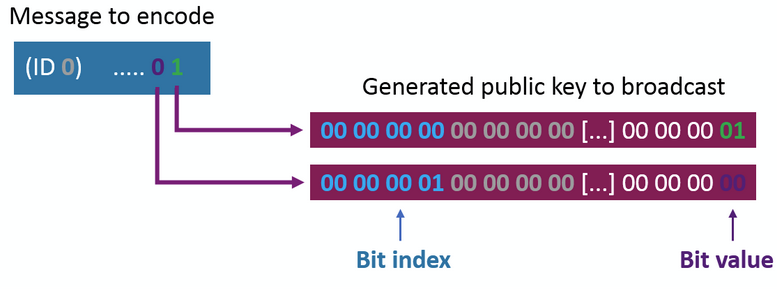
\includegraphics[width=0.9\linewidth]{sendmy_encoding.png}
  \caption{Bitweise Kodierung der Nachricht in im Advertisement übertragenen Daten \cite{braeunlein_sendmy}.}
  \label{fig:sendmy_encoding}
\end{figure}
Der Empfänger kann für jedes Bit der Nachricht die zwei möglichen Arrays generieren und eine Anfrage mit den jeweiligen \ac{SHA}-256 Hashes an Apples Server senden.
Abhängig davon, welcher der beiden Hashes in der Antwort enthalten ist, kann der Empfänger das Bit der Nachricht bestimmen.
Dabei wird ausgenutzt, dass jedes Apple Gerät die verschlüsselten Location Reports für beliebige öffentliche Schlüssel herunterladen kann.
Da die Location Reports Ende-zu-Ende verschlüsselt sind, wird dadurch die Vertraulichkeit nicht gefährdet.
Jedoch ist für dieses Missbrauchszenario die Entschlüsselung der Daten nicht notwendig, da lediglich das Vorhandensein eines bestimmten Location Reports überprüft werden muss, um die Nachricht zu dekodieren.
Ein Nachteil bei diesem Verfahren ist, dass somit auch jedes Apple-Gerät die Nachricht abrufen könnte.


Das von Tonetto \textit{et al.} \cite{Tonetto_FindMy} vorgestellte Verfahren verwendet 16 bekannten Advertising Keys, um die Nachricht in eine Folge dieser Keys zu kodieren.
Dazu wird eine Menge von Advertising Keys zuvor generiert und zwischen Sender und Empfänger ausgetauscht.
Der Sender kann die Nachricht erzeugt aus der Nachricht eine Abfolge der Advertising Keys und sendet diese nacheinander im Advertisement.
Finder Devices, die sich in der Nähe befinden, empfangen die Advertisements, erstellen Location Reports und laden diese hoch.
Der Empfänger der Nachricht kann alle Location Reports der bekannten Advertising Keys herunterladen, die Daten entschlüsseln und anhand der Zeitstempel die Folge und damit die ursprüngliche Nachricht rekonstruieren.
Im Vergleich zum Verfahren von Bräunlein, werden hier echte Advertising Keys verwendet, sodass die Location Reports entschlüsselt werden können, sodass der Standort des Senders bestimmt werden kann.
Zusätzlich muss der Empfänger weniger Anfragen an Apples Server stellen, da nur 16 unterschiedliche Advertising Keys verwendet werden.
Bräunleins Verfahren benötigt zwei Anfragen an Apples Server pro übertragenem Bit.


\subsection{M6: Korrelation von Standorten durch Apple}
\label{missbrauch:6}

Das zweite Ziel des Angreifermodells des Dienstanbieters (A4 in \autoref{fig:adversary_models}) bezieht sich auf die Korrelation von Standorten mehrerer Nutzer.
Heinrich \textit{et al.} \cite{Heinrich_FindMy} zeigen, dass durch den authentifizierten Up- und Download, die Korrelation durch Apple theoretisch möglich ist.
Die konkreten Standorte können aufgrund der Ende-zu-Ende-Verschlüsselung nicht bestimmt werden.
Allerdings kann bestimmt werden, welches Gerät welche Location Reports erstellt und welcher Nutzer diese heruntergeladen hat.
Daraus lässt sich folgern, welche Nutzer sich zu welcher Zeit an einem gemeinsamen Ort aufgehalten haben.
Apple könnte diese Informationen nutzen, um soziale Beziehungen zwischen Nutzern zu bestimmen und diese, zum Beispiel zu Werbezwecken, zu analysieren.
In \cite{Heinrich_FindMy} wird zusätzlich aufgezeigt, dass diese Daten auch von Strafverfolgungsbehörden genutzt werden könnten, um unter anderem die Identität von Demonstrationsteilnehmern zu bestimmen.
Jedoch ist nicht klar, ob Apple diese Daten tatsächlich speichert und nutzt.
\input{sections/gegenmaßnahmen.tex}
\section{Fazit}
\label{sec:Fazit}

% \subsubsection{Acknowledgements} Please place your acknowledgments at
% the end of the paper, preceded by an unnumbered run-in heading (i.e.
% 3rd-level heading).

\bibliographystyle{splncs04}
\bibliography{sources}

\end{document}
